\section{Systemarkitektur}
Dette afsnit omhandler de strukturelle rammer, som systemet blev lavet ud fra.

\subsection{Block Diagrammer}
De krav, der er stillet til systemet i projektoplægget - PSoC3 og DevKit8000 skal anvendes, der skal være bruger-interaktion, og der skal anvendes aktuatorer og følere til interaktion med omverdenen - førte til beslutningen om at systemet skulle kunne måle temperatur og luftfugtighed, og regulere disse igennem eksterne komponenter. Det blev også besluttet at systemet skulle kunne rotere emner ved hjælp af en stepmotor. Samtidig blev der truffet beslutning om, at DevKit8000 skulle benyttes til brugerinterface, og dermed være brugerens indgang til styring af systemet. PSoC3 skulle fungere som den regulerende, automatiserede del af systemet.

Til at illustrere disse valg blev der udarbejdet følgende logiske BDD:

\begin{figure}[H]
\centering
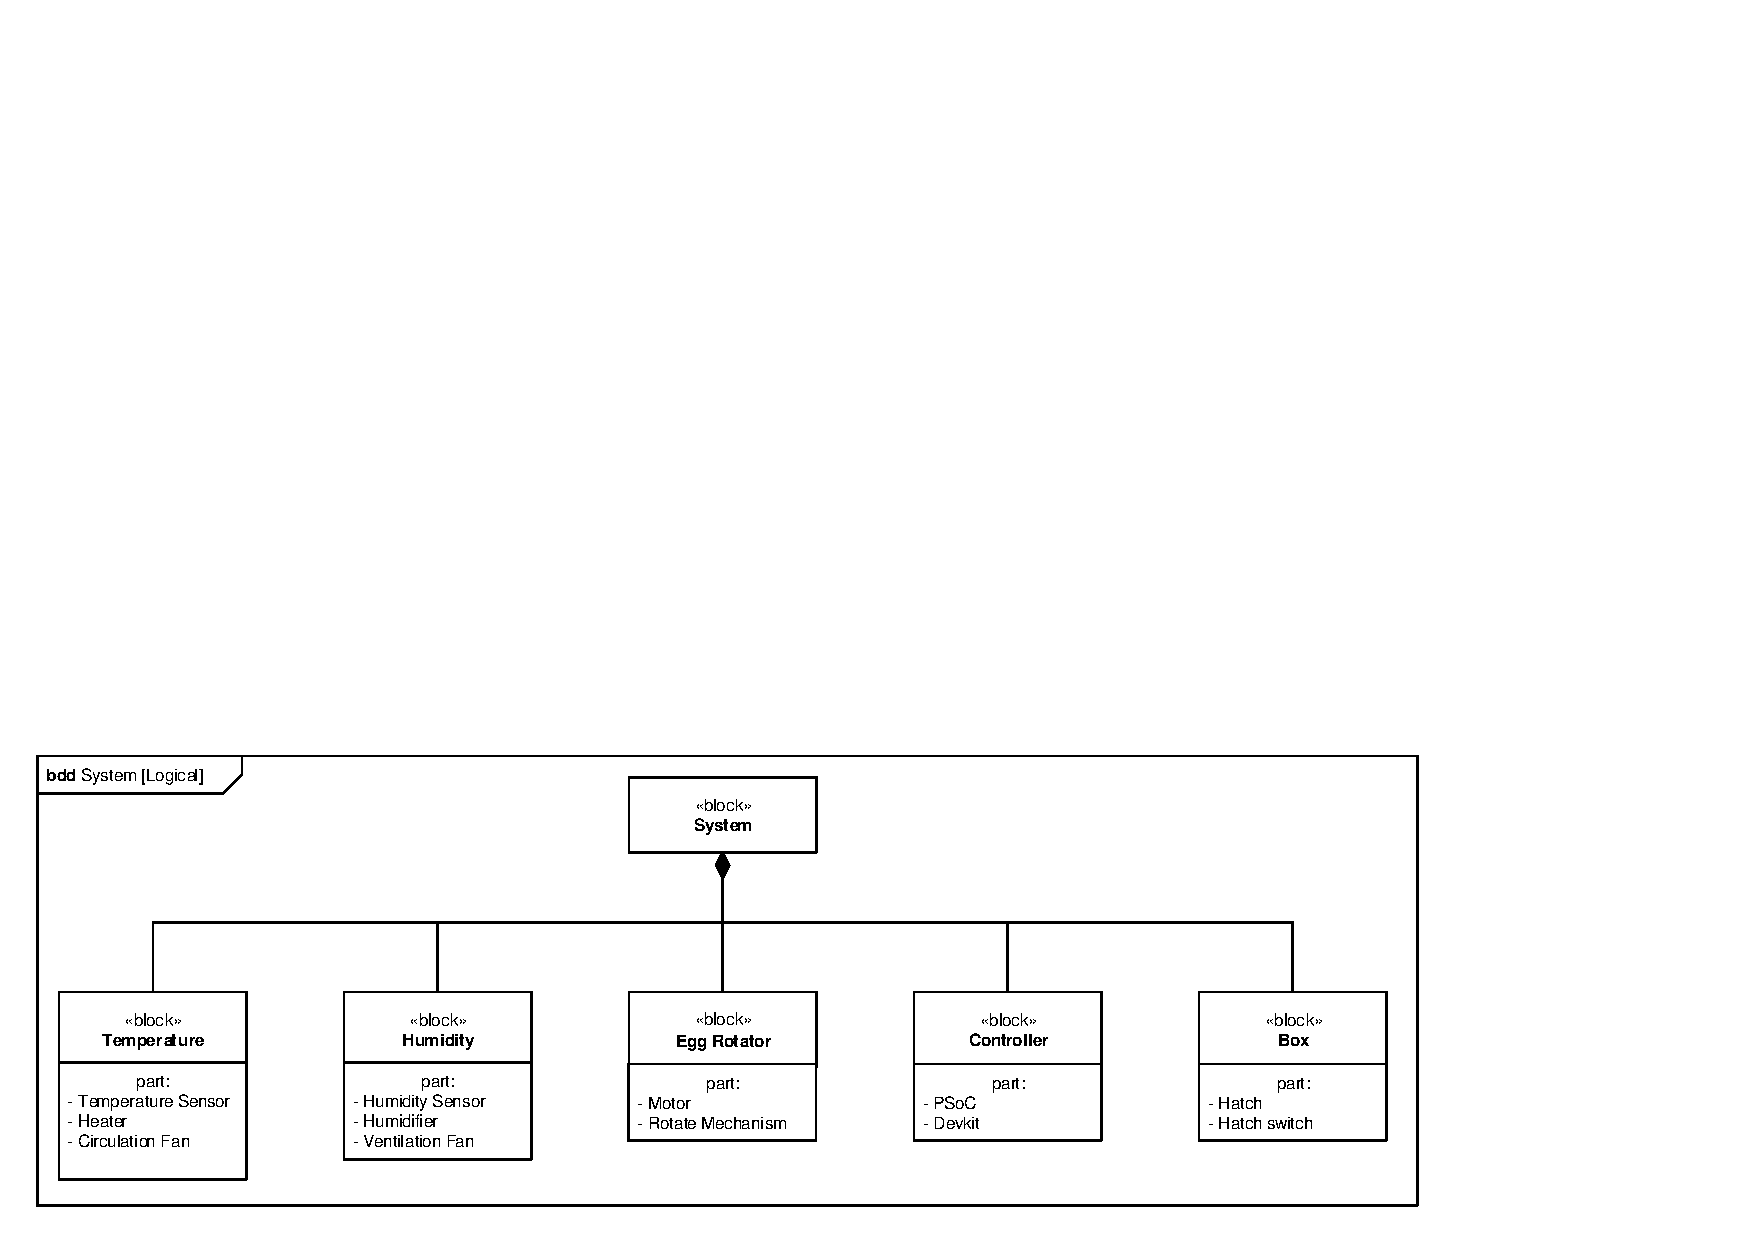
\includegraphics[width=\linewidth,page=1,trim=5mm 5mm 55mm 125mm]{./7_projektbeskrivelse/systemarkitektur/diagrammer/SYSML_Diagrammer_v4.pdf}
\caption[Diagram]{Logisk BDD for Systemet}
\label{fig:BDDLogisk}
\end{figure}
%scale=0.60,

Figur \ref{fig:BDDLogisk} viser de førnævnte dele samt nogle tilføjelser. For at opfylde krav om udluftning i Systemet er der blevet tilføjet en ventilations part under "Humidity" blokken, og for at nå en bedre varmefordeling er der ligeledes placeret en cirkulations part i "Heater" blokken.

"Box" blokken henviser til den fysiske rugekasse, der ikke er blevet lavet, og på samme måde henviser "Rotate Mechanism" parten i "Egg Rotator" blokken til den fysiske mekanisme, der fysisk skulle rotere emner i rugekassen.

Systemet blev herefter delt op i to fysiske dele: En Master del, som udgøres af DevKit8000 alene, samt en Slave del, der udgøres af PSoC3, samt de dele den kontrollerer. Der blev også taget stilling til hvordan de forskellige elementer skulle interagere med hinanden og igennem hvilket type interface. Dette er opsumeret i følgende fysiske BDD:

\begin{figure}[H]
\centering
\includegraphics[page=2,width=\linewidth,trim=5mm 5mm 210mm 20mm]{./7_projektbeskrivelse/systemarkitektur/diagrammer/SYSML_Diagrammer_v4.pdf}
\caption[Diagram]{Fysisk BDD for Systemet}
\label{fig:BDDFysisk}
\end{figure}

Som det fremgår af Figur \ref{fig:BDDFysisk}, blev det besluttet at kommunikation imellem de to blokke, PSoC3 og DevKit8000, skulle ske igennem SPI. Dette valg blev truffet ud fra foregående erfaringer med at kommunikere imellem disse igennem dette interface, opnået i forbindelse med andre opgaver. Som det også fremgår, blev det ligeledes besluttet, at alle sensorer skulle være digitale, og at de skulle være af I2C typen, da det ligeledes var noget vi havde erfaring med gennem tidligere opgaver.

Siden systemet grundlæggende udvikles til at skulle kunne håndtere forskellige typer af æg, der evt. har forskellige krav til omgivelsernes temperatur, blev det også valgt at den styrende udgang til varmeregulering skulle være af en velkendt, variabel type, og her faldt valget på et PWM signal.

For flere detaljer omkring de interne forbindelser henvises til IBD'erne i dokumentationen.
\clearpage
\subsection{Software Diagrammer}

Fra Use Casene blev den grundlæggende software arkitektur fastlagt ved brug af de sædvanlige metoder; domæne-modeller, sekvens- og klasse-diagrammer og state machines. 

På Figur \ref{fig:StateMachine} ses state machine diagrammet for systemet, som giver et overblik over opførelsen af systemet. 

\begin{figure}[H]
\centering
\includegraphics[page=3,scale=0.85,trim=5mm 5mm 230mm 190mm]{./7_projektbeskrivelse/systemarkitektur/diagrammer/ArkitekturDiagrammer.pdf}
\caption[Diagram]{State Machine for Systemet}
\label{fig:StateMachine}
\end{figure}

På Figur \ref{fig:KlasseDiagram} ses klassediagrammet, som viser de funktioner, der skal implementeres:

\begin{figure}[H]
\centering
\fbox{\includegraphics[page=4,scale=0.9,trim=5mm 5mm 100mm 230mm]{./7_projektbeskrivelse/systemarkitektur/diagrammer/ArkitekturDiagrammer.pdf}}
\caption[Diagram]{Klassediagram for Systemet}
\label{fig:KlasseDiagram}
\end{figure}

Det er værd at bemærke, at hovedparten af dette software afvikles på PSoC3.

For sekvensdiagrammerne henvises til dokumentationen.
